% ============================================================
% M2 轮4 S3 · 练习件 第10课时（1.2.5 空间中的距离）
% 题面：照题面库 成卷/题面库/课时10-1.2.5.md 全 16 题冻结入卷（卷面题号＝库序 1~16，组名已正名照登）；
%       组名/难度照库头第 3/4 字段（题4/5/6 暂定档「简单＊」经义-6 全量亲算判简单一致，标「简单」）。
% 模板基线＝练习线样张（六宏零改动拷入，qp-blocks 21327B）；版式＝练习线 p2 课时训练
%       （\keshi＋multicols＋花形三档 基础巩固1~10／综合提升11~14／思维探索15~16）。
% 图源：题2＝单元7 image2 → figs/dy7_image2.png（28mm，题干后选项前）；
%       题9＝讲练下 image127 → figs/jx_image127.png（25mm，题干后）；
%       题10＝讲练下 image151 → figs/jx_image151.png（32mm，题干后）。
%       题13/14 教材 C 组题面库冻结无【图】占位（照冻结态入卷）。
%       【装配轮0912】#14 删语曾随拓-057 删语作一致性延伸；后拓-057 改判整题撤重（批3 §四-13③），
%       延伸前提消失→#14 回冻照批3 §三-2 原口径（保留「如图所示，」），与同页 #13 同制。
%       【目验修红0913】装配本逐页目验逮出后主会话统一裁「删语、同先例」：#4/#13/#14 题首「如图所示，」
%       三处全删（题面文字自足可解；先例＝拓-046/047/058），#13/#14 随批3 §三-2 冻结登记**销冻结**，
%       #14 的 0912「回冻」口径就此废止；#4 系目验新逮（原不在图债登记内）。题面库
%       `成卷/题面库/课时10-1.2.5.md` 同三题同步删语并各挂【清稿注】，md／tex 双侧一致。
% 组装病预防（承批1修复法）：双位题号选项网格 0.5\linewidth-0.5\lxhang-0.25em／四连排
%       0.25\linewidth-0.25\lxhang-0.25em；\xiexwei 全体 minus 3mm 弹性；图行 penalty 链按批1 §五-9。
% 取值/组名照登对照/图位/登记事项：见 ../批3值台账.md 课时10 节。
% 编译：xelatex main.tex（两遍）→ python render.py → png/pageN.png
% ============================================================
\documentclass[fontset=none]{ctexart}
\usepackage{qp-m3} % 换装：六宏→qp-m3 单包（钉后版 md5 7c3930362be8a0a2bdf21bbf8ac16573，两补钉随版）

% ============================================================
% 练习件局部宏（照练习线样张页2形制搬入；本段只加件，不改件）
% ============================================================
\renewcommand{\qpjianming}{练习件}
\renewcommand{\qpceming}{高中数学\quad 选择性必修第一册(人教B版)} % 换装回钉：qp-m3 默认册名＝选必二，防页脚漂移（试迁规约·试迁报告§四 B3 实证必改）
\renewcommand{\qpzhangming}{第一章\quad 空间向量与立体几何}

% ---------- YJ-01 灰块页脚·练习册档（块 31.0×7.8mm，照练习线样张 31.0mm 修正版） ----------
\newcommand{\qpxsyema}{\ifnum\value{page}<10 00\fi\ifnum\value{page}>9 \ifnum\value{page}<100 0\fi\fi\arabic{page}}
\newcommand{\lxshuziL}{\hbox to 13.8mm{\setlength{\fboxsep}{0pt}\colorbox{pnumbg}{%
  \makebox[31.0mm][l]{\rule[-3.145mm]{0pt}{7.8mm}\hspace{2.8mm}\fontsize{10.7pt}{13pt}\selectfont\color{black}\numpnum\qpxsyema}}\hss}}
\newcommand{\lxshuziR}{\hbox to 13.8mm{\kern-17.2mm\setlength{\fboxsep}{0pt}\colorbox{pnumbg}{%
  \makebox[31.0mm][r]{\rule[-3.145mm]{0pt}{7.8mm}\fontsize{10.7pt}{13pt}\selectfont\color{black}\numpnum\qpxsyema\hspace{2.75mm}}}}}
\fancyfoot[RO]{\raisebox{-1.24mm}[0pt][0pt]{\qphuitext\qpzhangming\quad{\heiti\qpjianming}\hspace{3mm}\lxshuziL}}
\fancyfoot[LE]{\raisebox{-1.24mm}[0pt][0pt]{\lxshuziR\hspace{3mm}\qphuitext\qpceming}}

% ---------- HX-01 花形·三档名（练习册版 25.5×6.8mm，重叠 o＝5.1mm） ----------
% 局部宏 \huadianOverlapLx 已由 qp-m3 收编（等值定义），依换装方案§1.4 预删防撞名
% 局部宏 \dangbadge 已由 qp-m3 收编（等值定义），依换装方案§1.4 预删防撞名

% ---------- TJ-02 练习册悬挂题号（单号 5.75mm／双位 7.6mm） ----------
% 长度 \lxhang 已由 qp-m3 分配，预删防重复定义
% 局部宏 \tihao 已由 qp-m3 收编（等值定义），依换装方案§1.4 预删防撞名
% 局部宏 \lxopt 已由 qp-m3 收编（等值定义），依换装方案§1.4 预删防撞名
% 局部宏 \xiexwei 已由 qp-m3 收编（等值定义），依换装方案§1.4 预删防撞名
% 局部宏 \zu 已由 qp-m3 收编（等值定义），依换装方案§1.4 预删防撞名

\begin{document}
%成书重装五本跨本连续页码（G7方案B，承M2/M3装配先例）setcounter 注入位
\setcounter{page}{78}

% ============================================================
% 课时训练（三档 10＋4＋2＝16 题）
% ============================================================
\keshi{第10课时\quad 空间中的距离}
\begin{multicols}{2}
\emergencystretch=1em

\dangbadge{基}{础}{巩}{固}

\tihao{1}\zu{K1 点面距×坐标直套公式单选〔代表〕} \tieside{简单}已知点\(M(0,1,-2)\)，平面\(\alpha\)过原点，且垂直于向量\(\overrightarrow{n}=(1,-2,2)\)，则点\(M\)到平面\(\alpha\)的距离为\nobreak(\kongwei)
\lxopt{\makebox[\dimexpr0.25\linewidth-0.25\lxhang-0.25em\relax][l]{A．\(\sqrt{3}\)；}\makebox[\dimexpr0.25\linewidth-0.25\lxhang-0.25em\relax][l]{B．\(2\)；}\makebox[\dimexpr0.25\linewidth-0.25\lxhang-0.25em\relax][l]{C．\(6\)；}\makebox[\dimexpr0.25\linewidth-0.25\lxhang-0.25em\relax][l]{D．\(\sqrt{6}\)}}
\begin{ansblock}[练-课时10-1]
% ans:练-课时10-1
\ansitem{1}{B（d=2）}
\end{ansblock}

\tihao{2}\zu{K1〔第2题〕点面距×长方体建系计算单选} \tieside{简单}如图，在长方体\(ABCD\text{-}\penalty100 A_1B_1C_1D_1\)中，\(AD=AA_1=1\)，\(AB=2\)，点\(E\)是棱\(AB\)的中点，则点\(E\)到平面\(ACD_1\)的距离为\nobreak(\kongwei)
\par\vspace{1.9mm}\penalty10000\noindent\makebox[\linewidth][c]{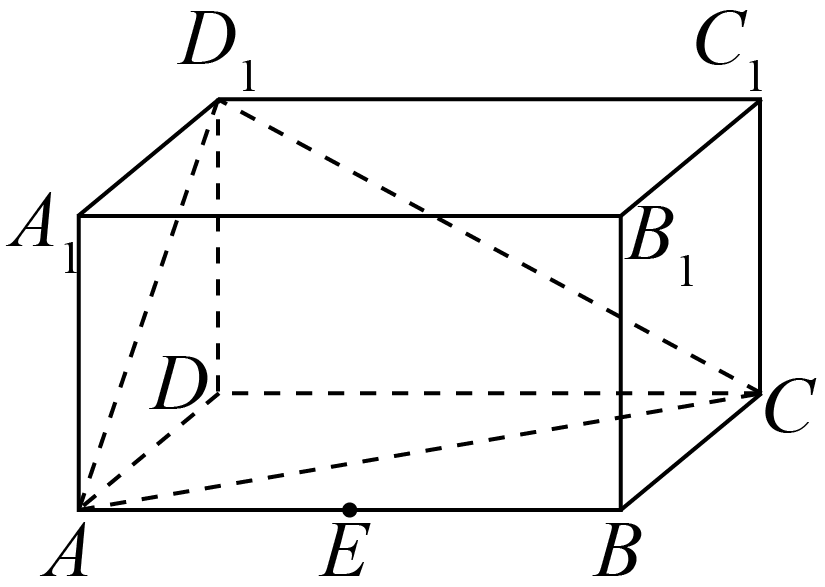
\includegraphics[width=28mm]{figs/dy7_image2.png}}\par\vspace{-1.0mm}\penalty10000
\lxopt{\makebox[\dimexpr0.25\linewidth-0.25\lxhang-0.25em\relax][l]{A．\(\frac{1}{2}\)；}\makebox[\dimexpr0.25\linewidth-0.25\lxhang-0.25em\relax][l]{B．\(\frac{\sqrt{2}}{2}\)；}\makebox[\dimexpr0.25\linewidth-0.25\lxhang-0.25em\relax][l]{C．\(\frac{1}{3}\)；}\makebox[\dimexpr0.25\linewidth-0.25\lxhang-0.25em\relax][l]{D．\(\frac{1}{6}\)}}
\begin{ansblock}[练-课时10-2]
% ans:练-课时10-2
\ansitem{2}{C（\(\dfrac{1}{3}\)）}
\ansnote{解析}{\(ACD_{1}\) 面 \(x-2y+2z=0\)，\(d=\dfrac{1}{3}\)。}
\end{ansblock}

\tihao{3}\zu{K2 点线距×已知坐标直取〔代表〕} \tieside{简单}已知\(A(0,0,2)\)，\(B(1,0,2)\)，\(C(0,2,0)\)，则点\(A\)到直线\(BC\)的距离为\nobreak(\kongwei)
\lxopt{\makebox[\dimexpr0.25\linewidth-0.25\lxhang-0.25em\relax][l]{A．\(\frac{2\sqrt{2}}{3}\)；}\makebox[\dimexpr0.25\linewidth-0.25\lxhang-0.25em\relax][l]{B．\(1\)；}\makebox[\dimexpr0.25\linewidth-0.25\lxhang-0.25em\relax][l]{C．\(\sqrt{2}\)；}\makebox[\dimexpr0.25\linewidth-0.25\lxhang-0.25em\relax][l]{D．\(2\sqrt{2}\)}}
\begin{ansblock}[练-课时10-3]
% ans:练-课时10-3
\ansitem{3}{A（\(\dfrac{2\sqrt{2}}{3}\)）}
\ansnote{解析}{\(|\overrightarrow{BA}\times\overrightarrow{BC}|=2\sqrt{2}\)、\(|BC|=3\)；向量坐标不加模线。}
\end{ansblock}

\tihao{4}\zu{K3 定点到定直线段距离×正三角形中心垂线} \tieside{简单}已知正三角形\(ABC\)的中心为\(O\)，\(OP\perp\)平面\(ABC\)且\(AB=2OP=2\,\mathrm{cm}\)，求点\(P\)到这个正三角形各边的距离．
\xiexwei{20mm}
\begin{ansblock}[练-课时10-4]
% ans:练-课时10-4
\ansitem{4}{\(\dfrac{2\sqrt{3}}{3}\) cm}
\end{ansblock}

\tihao{5}\zu{K4 墙角三面垂直×等体积法点面距} \tieside{简单}已知三棱锥\(O\text{-}\penalty100 ABC\)中，\(OA\)，\(OB\)，\(OC\)的长度均为\(2\)，且两两互相垂直，求点\(O\)到平面\(ABC\)的距离．
\xiexwei{20mm}
\begin{ansblock}[练-课时10-5]
% ans:练-课时10-5
\ansitem{5}{\(\dfrac{2\sqrt{3}}{3}\)}
\end{ansblock}

\tihao{6}\zu{K5〔第2题〕正方体点面距＋面面距题组} \tieside{简单}已知正方体\(ABCD\text{-}\penalty100 A'B'C'D'\)的棱长为\(1\)．
\lxopt{(1)求\(B'\)到平面\(A'C'B\)的距离；}
\lxopt{(2)求平面\(A'C'B\)与平面\(D'AC\)之间的距离．}
\xiexwei{24mm}
\begin{ansblock}[练-课时10-6]
% ans:练-课时10-6
\ansitem{6}{(1)\(\dfrac{\sqrt{3}}{3}\)；(2)\(\dfrac{\sqrt{3}}{3}\)}
\end{ansblock}

\tihao{7}\zu{K8 等体积法×内切球半径〔代表〕（\(r=\frac{h}{4}\) 公式直取）} \tieside{简单}棱长为\(a\)的正四面体的内切球半径为\kongbai{}．
\begin{ansblock}[练-课时10-7]
% ans:练-课时10-7
\ansitem{7}{\(\dfrac{\sqrt{6}a}{12}\)}
\end{ansblock}

\tihao{8}\zu{K8〔第2题〕升维类比 3\(\to\)4（详解直引 -33 公式）} \tieside{简单}“正三角形的内切圆半径等于此正三角形的高的\(\frac{1}{3}\)”，拓展到空间，类比平面几何的上述结论，则正四面体的内切球半径等于这个正四面体的高的\nobreak(\kongwei)
\lxopt{\makebox[\dimexpr0.25\linewidth-0.25\lxhang-0.25em\relax][l]{A．\(\frac{1}{2}\)；}\makebox[\dimexpr0.25\linewidth-0.25\lxhang-0.25em\relax][l]{B．\(\frac{1}{3}\)；}\makebox[\dimexpr0.25\linewidth-0.25\lxhang-0.25em\relax][l]{C．\(\frac{1}{4}\)；}\makebox[\dimexpr0.25\linewidth-0.25\lxhang-0.25em\relax][l]{D．\(\frac{1}{5}\)}}
\begin{ansblock}[练-课时10-8]
% ans:练-课时10-8
\ansitem{8}{C（\(\dfrac{1}{4}\)）}
\end{ansblock}

\tihao{9}\zu{K4〔第2题〕点线＋点面双问×正三棱柱建系大题} \tieside{中档}如图，正三棱柱\(ABC\text{-}\penalty100 A_1B_1C_1\)中，各棱长均为\(4\)，\(N\)是\(CC_1\)的中点．
\par\vspace{1.9mm}\penalty10000\noindent\makebox[\linewidth][c]{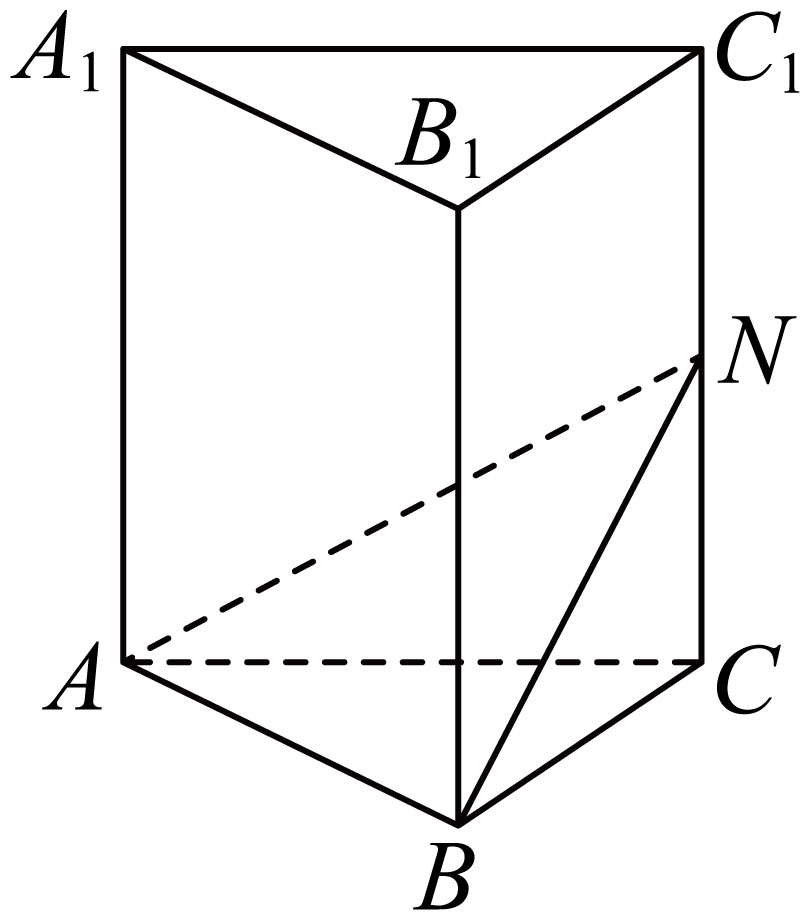
\includegraphics[width=25mm]{figs/jx_image127.png}}\par\vspace{-1.0mm}\penalty10000
\lxopt{(1)求点\(N\)到直线\(AB\)的距离；}
\lxopt{(2)求点\(C_1\)到平面\(ABN\)的距离．}
\xiexwei{36mm}
\begin{ansblock}[练-课时10-9]
% ans:练-课时10-9
\ansitem{9}{(1)\(4\)；(2)\(\sqrt{3}\)}
\end{ansblock}

\tihao{10}\zu{K5b 线面距×五面体（定义法综合路）〔代表〕} \tieside{中档}如图，在五面体\(ABCDEF\)中，\(AB\parallel DC\)，\(\angle BAD=\frac{\pi}{2}\)，\(CD=AD=2\)，四边形\(ABFE\)为平行四边形，\(FA\perp\)平面\(ABCD\)，\(FC=3\)，\(ED=\sqrt{7}\)．
\par\vspace{1.9mm}\penalty10000\noindent\makebox[\linewidth][c]{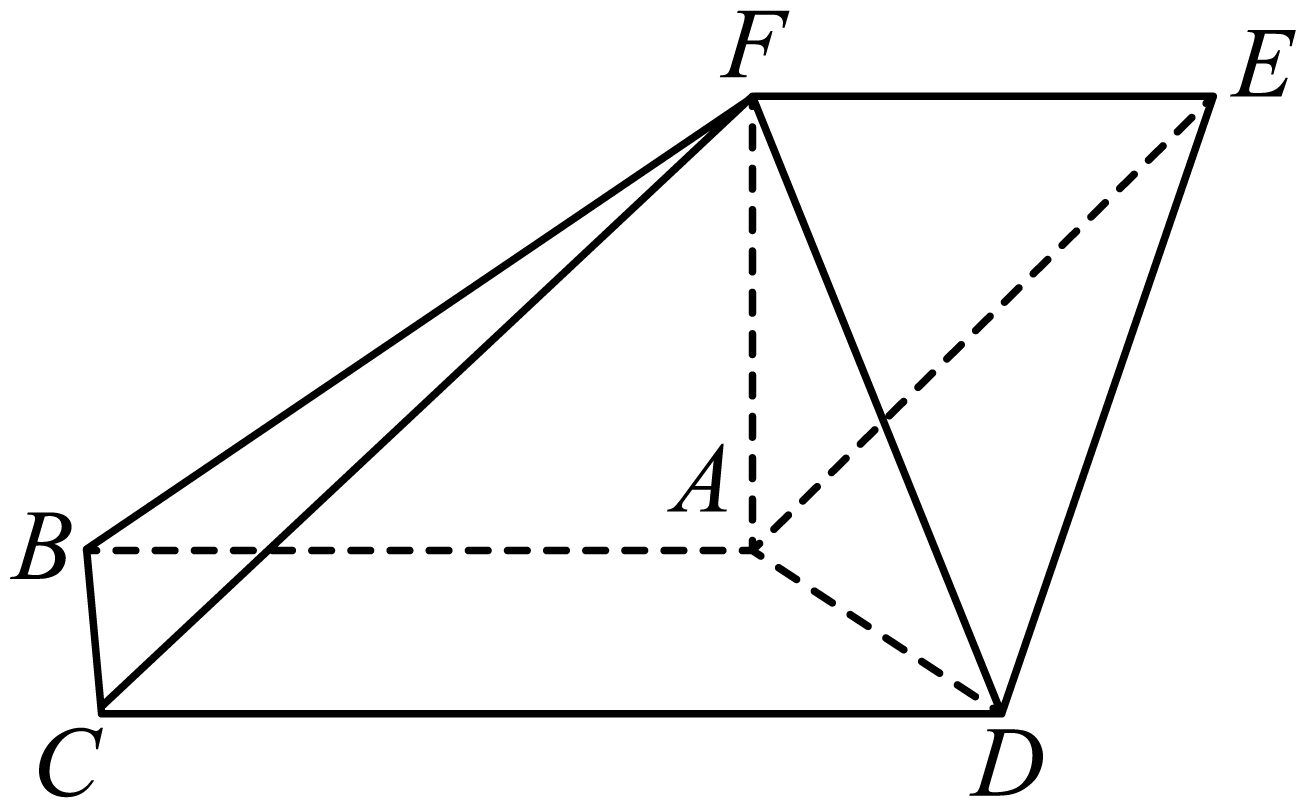
\includegraphics[width=32mm]{figs/jx_image151.png}}\par\vspace{-1.0mm}\penalty10000
\lxopt{(1)求直线\(AB\)到平面\(EFCD\)的距离；}
\lxopt{(2)求二面角\(F\text{-}\penalty100 AD\text{-}\penalty100 E\)的平面角的正切值．}
\xiexwei{44mm}
\begin{ansblock}[练-课时10-10]
% ans:练-课时10-10
\setlength{\anshang}{7.6mm}% 题10 起双位档（照答案册同值，块内局部）
\ansitem{10}{(1)\(\dfrac{2\sqrt{5}}{5}\)；(2)\(\sqrt{2}\)}
\end{ansblock}

\dangbadge{综}{合}{提}{升}

\tihao{11}\zu{K6 异面直线距离×补形正方体（基准⑤唯一主干件）} \tieside{中档}已知四面体\(SABC\)的所有棱长均为\(10\)，点\(P\)在直线\(AS\)上，则\(P\)到\(BC\)的距离的最小值为\nobreak(\kongwei)
\lxopt{\makebox[\dimexpr0.25\linewidth-0.25\lxhang-0.25em\relax][l]{A．\(\frac{5\sqrt{2}}{2}\)；}\makebox[\dimexpr0.25\linewidth-0.25\lxhang-0.25em\relax][l]{B．\(\frac{10\sqrt{3}}{3}\)；}\makebox[\dimexpr0.25\linewidth-0.25\lxhang-0.25em\relax][l]{C．\(5\sqrt{2}\)；}\makebox[\dimexpr0.25\linewidth-0.25\lxhang-0.25em\relax][l]{D．\(\frac{20\sqrt{3}}{3}\)}}
\begin{ansblock}[练-课时10-11]
% ans:练-课时10-11
\setlength{\anshang}{7.6mm}% 题11 起双位档（照答案册同值，块内局部）
\ansitem{11}{C（\(5\sqrt{2}\)）}
\end{ansblock}

\tihao{12}\duoxuan\zu{K5 距离公式选择·一题四距全覆盖×多选（组骨）} \tieside{中档}已知正方体\(ABCD\text{-}\penalty100 A_1B_1C_1D_1\)的棱长为\(1\)，点\(E\)，\(O\)分别是\(A_1B_1\)，\(A_1C_1\)的中点，\(P\)在正方体内部且满足\(\overrightarrow{AP}=\frac{3}{4}\overrightarrow{AB}+\frac{1}{2}\overrightarrow{AD}+\frac{2}{3}\overrightarrow{AA_1}\)，则下列说法正确的是\nobreak(\kongwei)
\lxopt{A．点\(A\)到直线\(BE\)的距离是\(\frac{\sqrt{5}}{5}\)；}
\lxopt{B．点\(O\)到平面\(ABC_1D_1\)的距离为\(\frac{\sqrt{2}}{4}\)；}
\lxopt{C．平面\(A_1BD\)与平面\(B_1CD_1\)间的距离为\(\frac{\sqrt{3}}{3}\)；}
\lxopt{D．点\(P\)到直线\(AB\)的距离为\(\frac{25}{36}\)}
\begin{ansblock}[练-课时10-12]
% ans:练-课时10-12
\setlength{\anshang}{7.6mm}% 题12 起双位档（照答案册同值，块内局部）
\ansitem{12}{BC}
\ansnote{解析}{D 项 \(\dfrac{5}{6}\)（嵌套绝对值与括号易错）。}
\end{ansblock}

\tihao{13}\zu{异面直线所成角×坐标法三小问×解答（C组难档槽位，亲判简单偏中档）} \tieside{难}已知四棱锥\(P\text{-}\penalty100 ABCD\)中，\(ABCD\)为矩形，\(PD\perp\)平面\(ABCD\)，\(PD=3\)，\(AB=5\)，\(BC=4\)，求下列各对异面直线所成角的余弦值：
\lxopt{(1)\(PC\)与\(AB\)；}
\lxopt{(2)\(PD\)与\(AB\)；}
\lxopt{(3)\(PA\)与\(BC\)．}
\xiexwei{64mm}
\begin{ansblock}[练-课时10-13]
% ans:练-课时10-13
\setlength{\anshang}{7.6mm}% 题13 起双位档（照答案册同值，块内局部）
\ansitem{13}{(1)\(\dfrac{5\sqrt{34}}{34}\)；(2)\(0\)；(3)\(\dfrac{4}{5}\)}
\end{ansblock}

\tihao{14}\zu{线面角×定比分点×三垂线综合×解答（C组难档槽位，亲判中档偏上）} \tieside{难}直三棱柱\(ABC\text{-}\penalty100 A_1B_1C_1\)中，\(AC\perp BC\)，点\(M\)在线段\(AB\)上，\(AC=BC=CC_1=3\)，\(AM=\sqrt{2}\)，求直线\(AC_1\)与平面\(B_1MC\)所成角的正弦值．
\xiexwei{84mm}
\begin{ansblock}[练-课时10-14]
% ans:练-课时10-14
\setlength{\anshang}{7.6mm}% 题14 起双位档（照答案册同值，块内局部）
\ansitem{14}{\(\dfrac{\sqrt{2}}{6}\)}
\end{ansblock}

\dangbadge{思}{维}{探}{索}

\tihao{15}\zu{空间距离·纯坐标直取（点线距/点面距）×选择〔代表〕} \tieside{简单}在空间直角坐标系\(O\text{-}\penalty100 xyz\)中，已知点\(C(2,1,2)\)，则点\(A(2,2,0)\)到直线\(OC\)的距离为\nobreak(\kongwei)
\lxopt{\makebox[\dimexpr0.25\linewidth-0.25\lxhang-0.25em\relax][l]{A．\(2\)；}\makebox[\dimexpr0.25\linewidth-0.25\lxhang-0.25em\relax][l]{B．\(\sqrt{2}\)；}\makebox[\dimexpr0.25\linewidth-0.25\lxhang-0.25em\relax][l]{C．\(2\sqrt{2}\)；}\makebox[\dimexpr0.25\linewidth-0.25\lxhang-0.25em\relax][l]{D．\(4\)}}
\begin{ansblock}[练-课时10-15]
% ans:练-课时10-15
\setlength{\anshang}{7.6mm}% 题15 起双位档（照答案册同值，块内局部）
\ansitem{15}{A（2）}
\end{ansblock}

\tihao{16}\zu{空间距离·纯坐标直取（点线距/点面距）〔第2题〕×填空} \tieside{简单}在空间直角坐标系\(O\text{-}\penalty100 xyz\)中，平面\(\alpha\)经过\(A(1,0,0)\)，\(B(0,1,0)\)，\(C(0,0,1)\)三点，点\(P(1,1,2)\)．则点\(P\)到平面\(\alpha\)的距离为\kongbai{}．
\begin{ansblock}[练-课时10-16]
% ans:练-课时10-16
\setlength{\anshang}{7.6mm}% 题16 起双位档（照答案册同值，块内局部）
\ansitem{16}{\(\sqrt{3}\)}
\ansnote{解析}{应为连线段 CP（\(\overrightarrow{CP}=(1,1,1)\parallel\overrightarrow{n}\) 实为垂线段），且垂足恰为 C，\(d=|PC|=\sqrt{3}\) 第二路可验。}
\end{ansblock}

\end{multicols}

\tailfill
\end{document}
